\def\fpn{
    Feature Pyramid Networks \cite{lin2017feature} (gọi tắt là FPN) được giới thiệu như một kiến trúc backbone trong các mô hình object detection nhằm giải quyết vấn đề chênh lệch về kích thước giữa các đối tượng trong ảnh.
    Việc sử dụng FPN như là kiến trúc backbone kết hợp cùng mô hình Faster R-CNN đã vượt qua rất nhiều các mô hình object detection khác để trở thành mô hình SOTA ở thời điểm đó.

    \noindent
    \textbf{\textit{So sánh các kiến trúc pyramid khác nhau}}

    \begin{figure}[H]
        \centering
        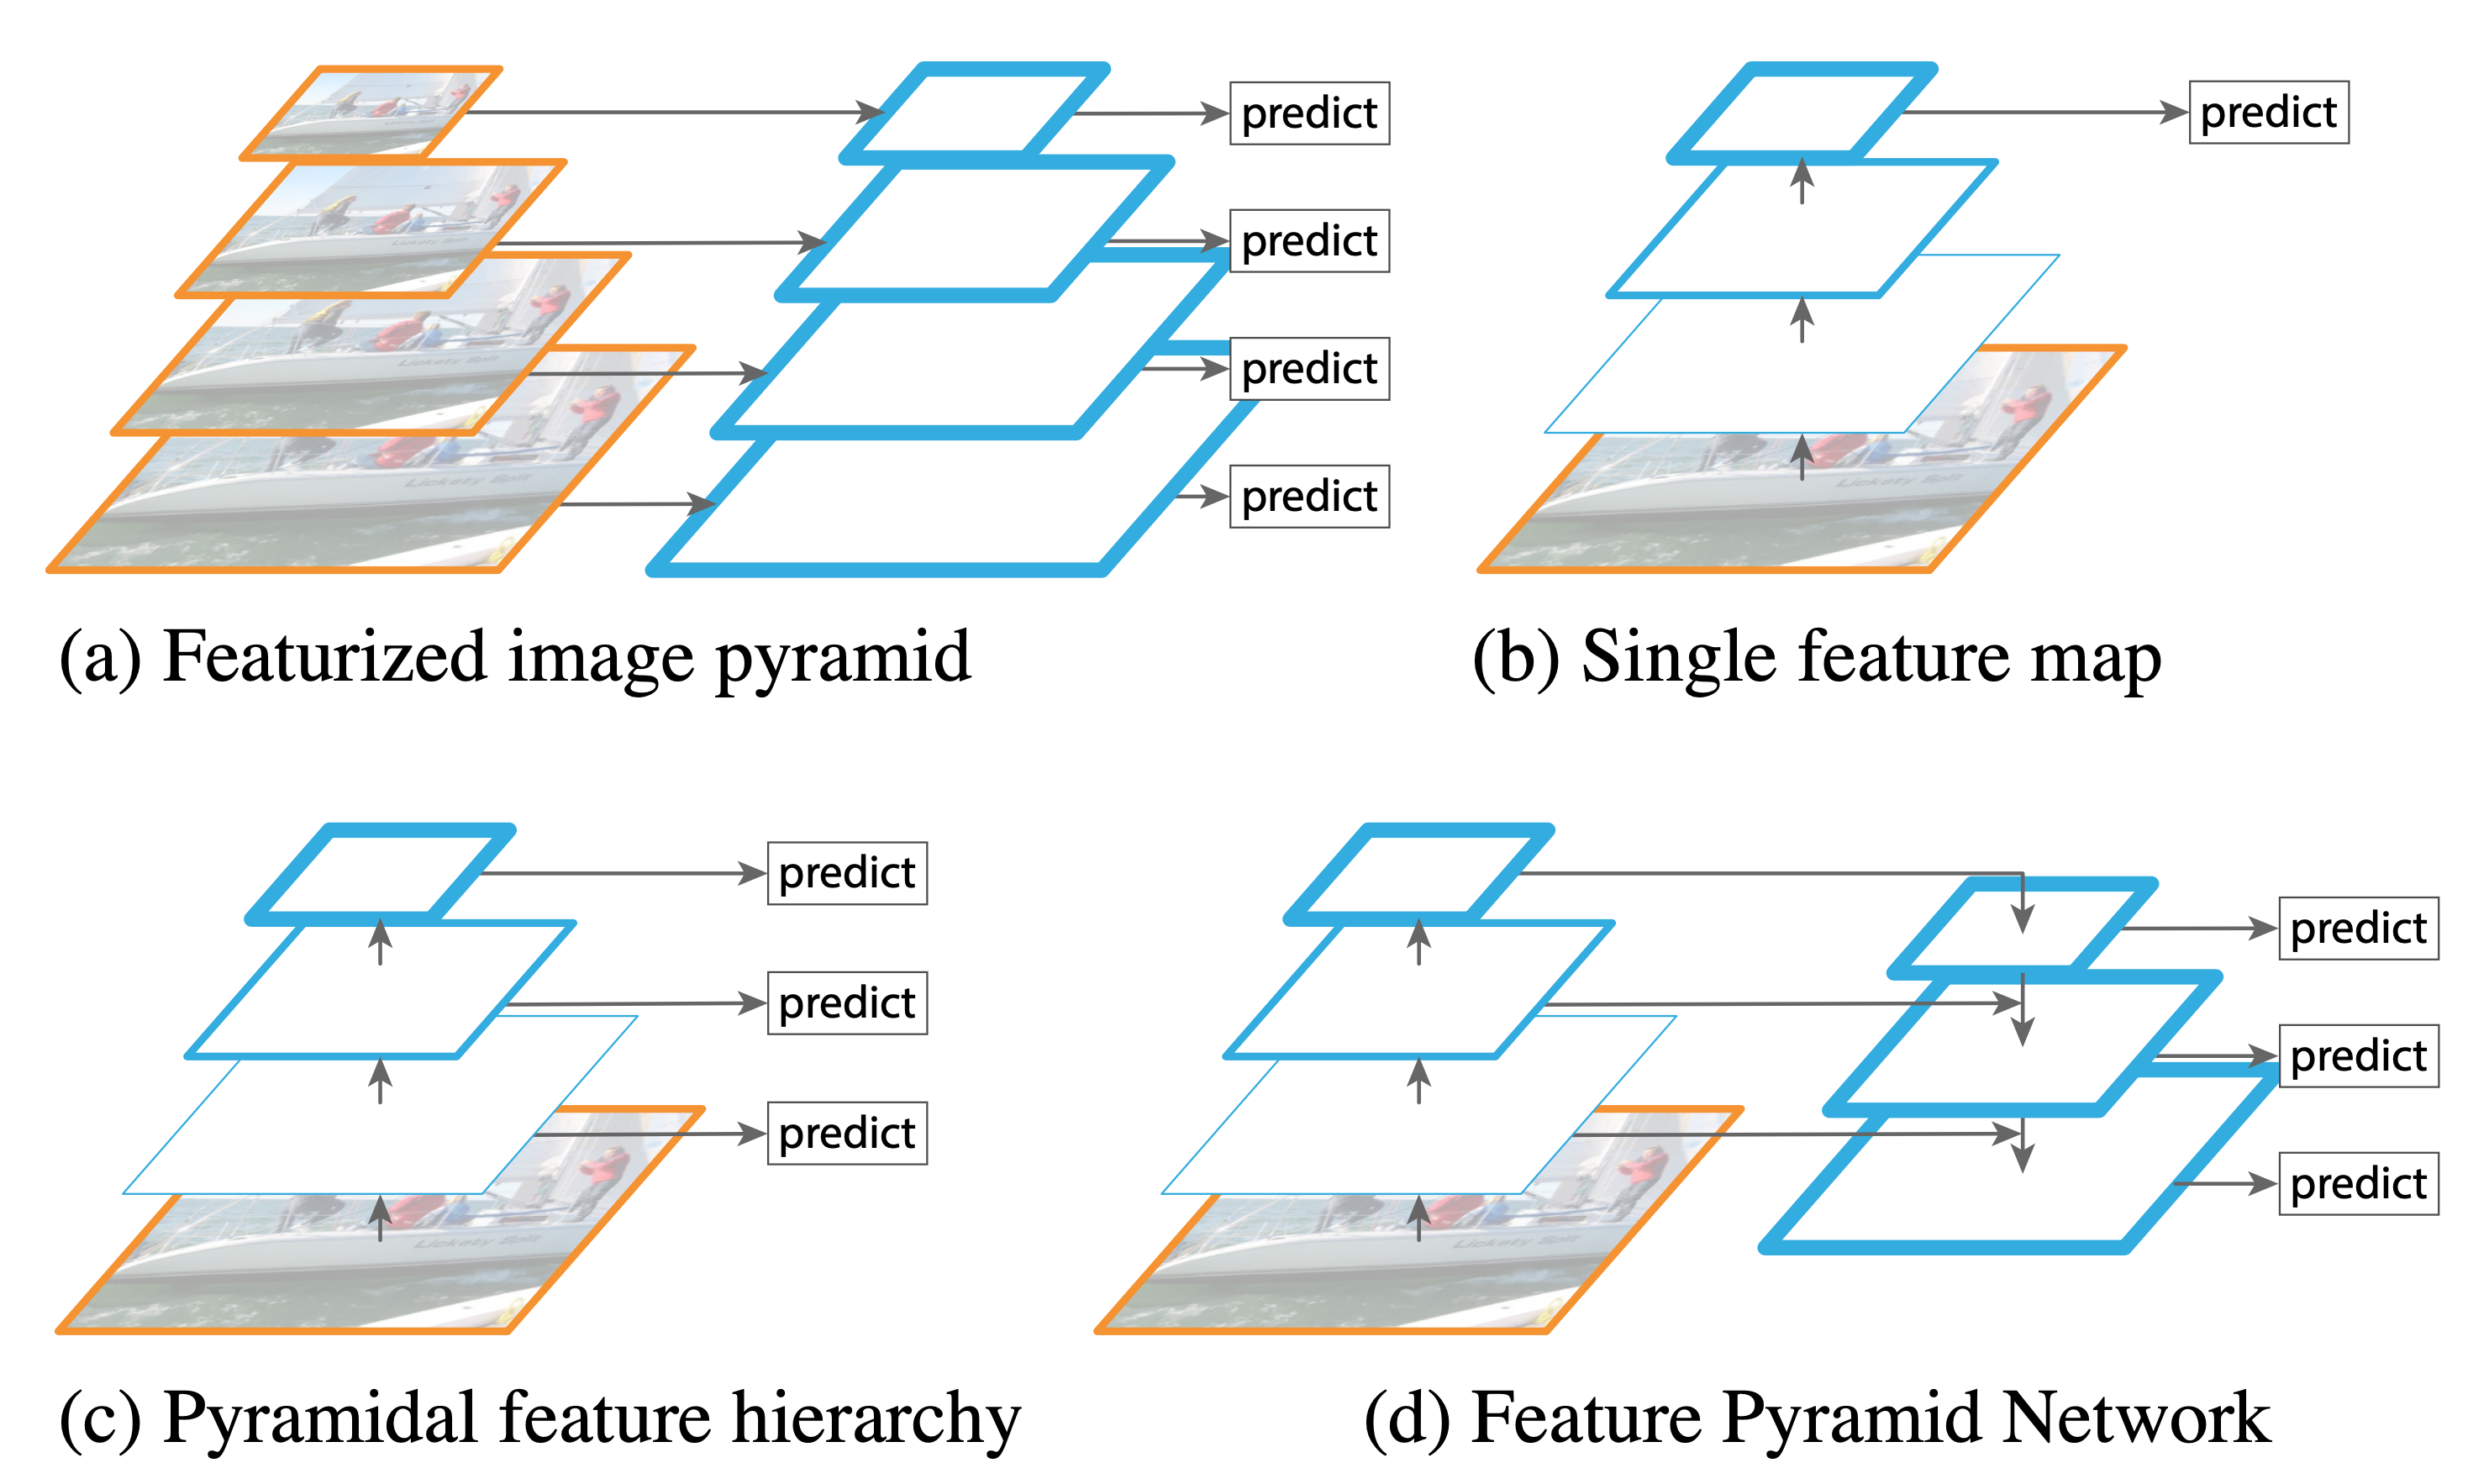
\includegraphics[width=11cm] {images/fpn_compare}
        \caption{So sánh các kiến trúc pyramid khác nhau (Nguồn: \cite{lin2017feature})}
        \label{fig:fpn_compare}
    \end{figure}

    \noindent
    Ý tưởng về việc xây dựng và sử dụng các đặc trưng của ảnh với nhiều kích thước khác nhau không mới, tuy nhiên, các giải pháp đã có vào thời điểm đó đều vướng phải một số vấn đề: \\
    - \textit{Featurized image pyramid}: Việc sử dụng nhiều kích thước ảnh khác nhau để tạo ra nhiều đặc trưng có kích thước khác nhau một cách độc lập là ý tưởng cơ bản nhất. Mặc dù đạt được hiệu quả cao về độ chính xác khi khai thác ảnh đầu vào với nhiều kích thước khác nhau, nhưng phương pháp này khiến cho mô hình giải bài toán object detection trở nên cồng kềnh và tốn rất nhiều thời gian để xử lý và gần như bất khả thi để có thể train được mô hình. \\
    - \textit{Single feature map}: Việc sử dụng chỉ một kích thước đặc trưng duy nhất giúp cho mô hình xử lý nhanh hơn nhưng lại khiến cho mô hình khó có thể học được những đặc trưng giữa các đối tượng có kích thước chênh lệch trong ảnh. Đặc biệt, việc đưa ảnh đầu vào qua nhiều khối Conv đã loại bỏ rất nhiều thông tin và gần như không còn thông tin để mô hình có thể nhận biết được các đối tượng có kích thước nhỏ. \\
    - \textit{Pyramidal feature hierarchy}: Việc sử dụng nhiều feature maps có kích thước khác nhau cùng đưa ra kết quả được sử dụng trong mô hình object detection khá nổi tiếng là SSD \cite{liu2016ssd}. Tuy nhiên, thay vì tận dụng toàn bộ các feature maps sinh ra từ các khối Conv của backbone VGG-16, SSD chỉ sử dụng feature map từ khối Conv thứ 5 và bổ sung thêm các lớp Conv. Điều này khiến cho SSD bỏ qua những feature map có kích thước lớn, có ý nghĩa quan trọng trong việc detect các đối tượng có kích thước nhỏ. \\
    - \textit{Feature Pyramid Network}: Dựa trên vấn đề trên từ SSD, nhóm tác giả đề xuất FPN tận dụng tối đa các feature maps trích xuất được từ backbone nhằm tạo ra bộ feature map mới gồm nhiều kích thước khác nhau và chứa rất nhiều thông tin về nội dung của ảnh đầu vào. Để đạt được điều này, nhóm tác giả thiết kế kiến trúc kết hợp những feature maps có kích thước lớn và những feature maps có kích thước nhỏ bằng top-down pathway và lateral connections.

    \noindent
    \textbf{\textit{Kiến trúc mô hình Feature Pyramid Networks}} \\
    Ý tưởng về việc sử dụng kiến trúc mô hình theo dạng top-down không phải là mới và đã được nhắc đến trong một số nghiên cứu. Tuy nhiên, điểm giống nhau của các nghiên cứu có thiết kế mô hình theo kiểu top-down đó là mô hình chỉ sử dụng một feature map cuối cùng, sau khi đã tổng hợp các thông tin trong suốt quá trình top-down, để đưa ra quyết định dự đoán cuối cùng.

    \noindent
    Trong khi đó, đối với FPN, nhóm tác giả đưa ra quyết định dự đoán trên từng feature maps trong suốt quá trình top-down. Từ đó, đặc biệt nâng cao chất lượng của mô hình object detection khi có thể vừa trích xuất được thông tin của các đối tượng có kích thước lớn từ các feature map có kích thước nhỏ vừa trích xuất được thông tin của các đối tượng có kích thước nhỏ từ các feature map có kích thước lớn.

    \begin{figure}[H]
        \centering
        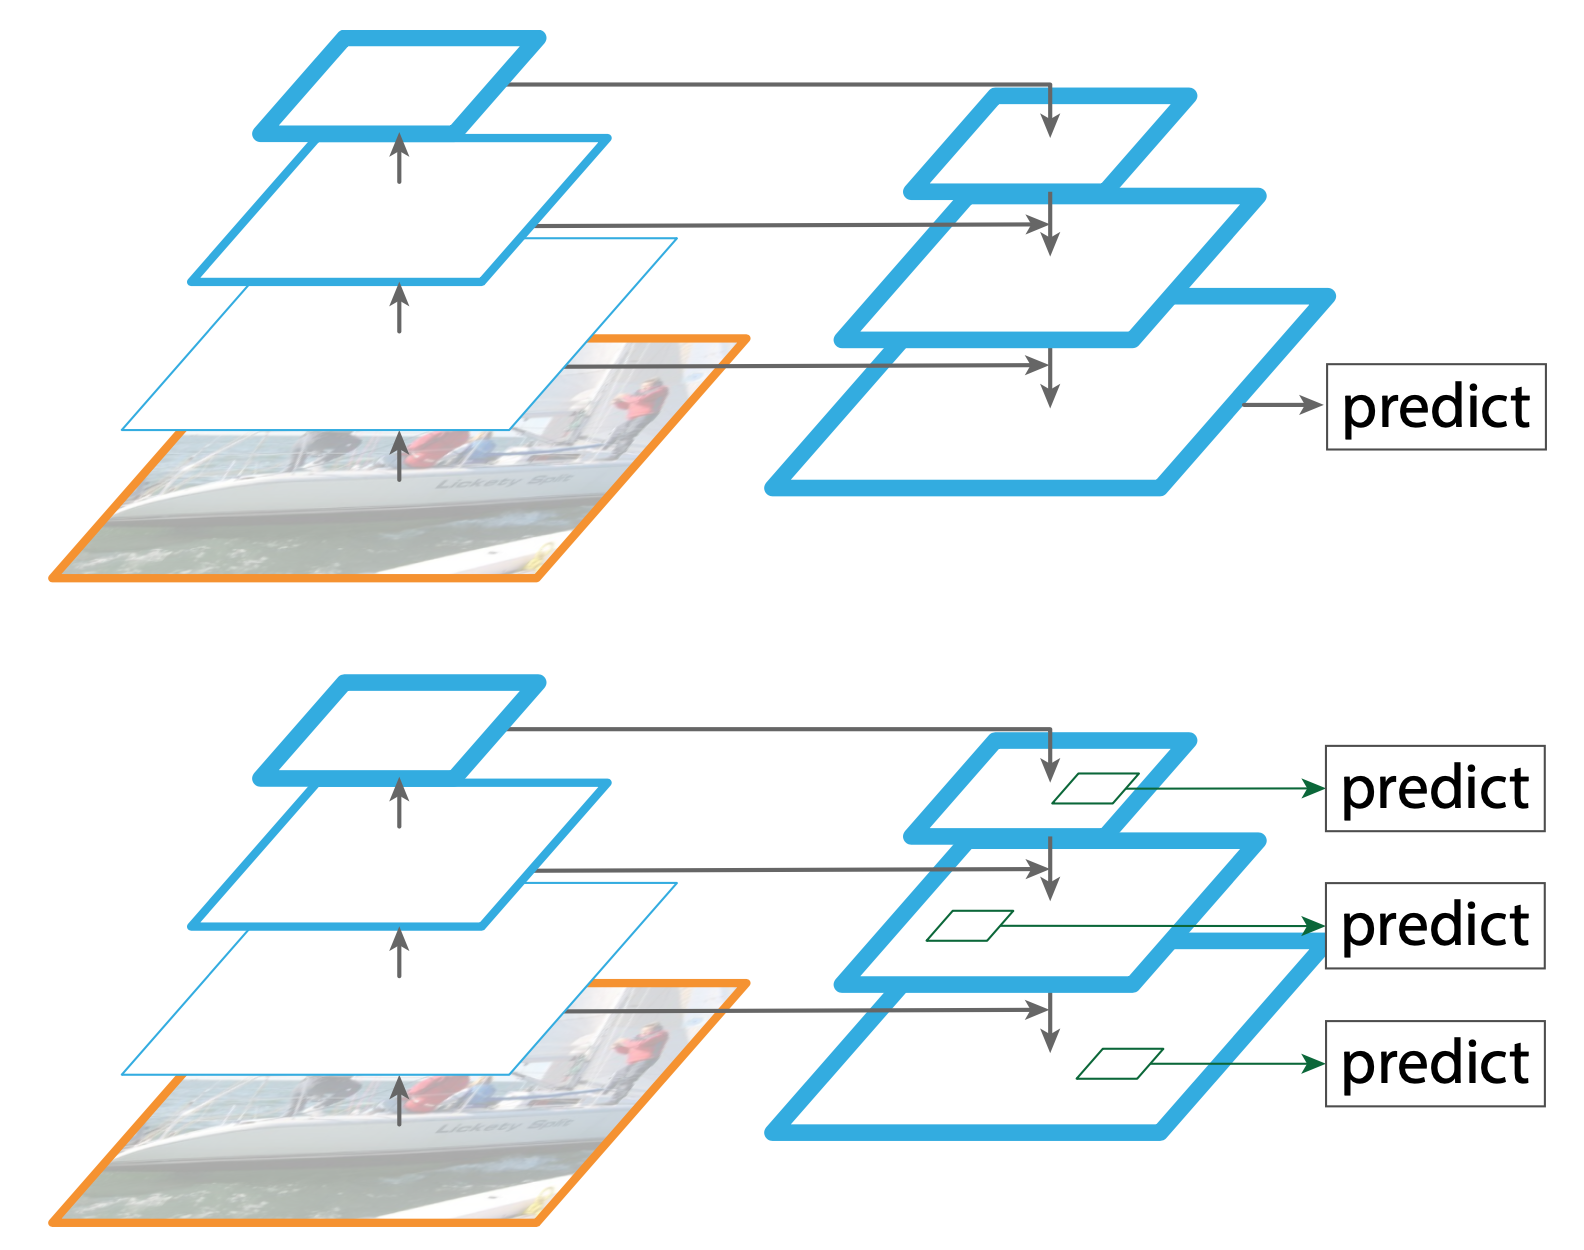
\includegraphics[width=6cm] {images/fpn_topdown}
        \caption{So sánh các kiến trúc theo dạng top-down khác nhau (Nguồn: \cite{lin2017feature})}
        \label{fig:fpn_topdown}
    \end{figure}

    \noindent
    Kiến trúc FPN có thể được áp dụng với nhiều backbone Conv khác nhau như AlexNet, VGG hay ResNet, cụ thể trong nghiên cứu, nhóm tác giả lựa chọn ResNet làm mô hình backbone.
    Kiến trúc FPN có thể được chia làm hai phần: \\
    - \textit{Bottom-up pathway} là quá trình mà ta đưa ảnh đầu vào qua mô hình backbone Conv như ResNet và thu được các feature map.
    Tuy nhiên, trong các mô hình backbone Conv, sẽ có một nhóm các lớp Conv tạo ra các feature map có kích thước giống nhau, và nhóm các lớp Conv này được gọi là một khối Conv.
    Đối với FPN, nhóm tác giả lựa chọn các feature map được sinh ra từ các lớp Conv cuối cùng trong mỗi khối Conv để sử dụng cho nhánh Top-down pathway.
    Cụ thể đối với mô hình backbone ResNet, nhóm tác giả sử dụng các feature maps được sinh ra từ residual block cuối cùng của mỗi khối Conv (trừ khối Conv đầu tiên do kích thước của feature maps này lớn và gây ra vấn đề về bộ nhớ), ký hiệu là \textit{{${C}_{2}, {C}_{3}, {C}_{4}, {C}_{5}$}}.
    Các feature maps này có kích thước lần lượt bằng 1/4, 1/8, 1/16 và 1/32 so với kích thước của ảnh đầu vào. \\
    - \textit{Top-down pathway và lateral connections} là quá trình mà FPN sinh ra thêm các feature maps mới từ các feature maps của Bottom-up pathway và kết hợp chúng lại thông qua lateral connections.
    Cụ thể, các feature maps của Bottom-up pathway được đưa qua các lớp Conv có kích thước 1x1, stride bằng 1 nhằm giữ nguyên kích thước chiều dài, chiều rộng và chỉ thay đổi kích thước chiều channel của feature maps.
    Các feature maps ở vị trí cao hơn (có kích thước nhỏ hơn) được upsample thông qua thuật toán nearest neighbor và cộng ma trận với feature maps đầu ra từ lớp Conv 1x1 nói trên.
    Cuối cùng, các feature maps đầu ra từ phép cộng ma trận nói trên được đi qua một lớp Conv 3x3 có cùng số đầu ra channel của feature maps nhằm giảm bớt hiệu ứng của thuật toán nearest neighbor và tạo ra các feature maps đầu ra cuối cùng có cùng số channel với nhau.
    Tập hợp feature maps này được gọi là \textit{{${P}_{2}, {P}_{3}, {P}_{4}, {P}_{5}$}} tương ứng với các feature maps có cùng kích thước \textit{{${C}_{2}, {C}_{3}, {C}_{4}, {C}_{5}$}}.

    \begin{figure}[H]
        \centering
        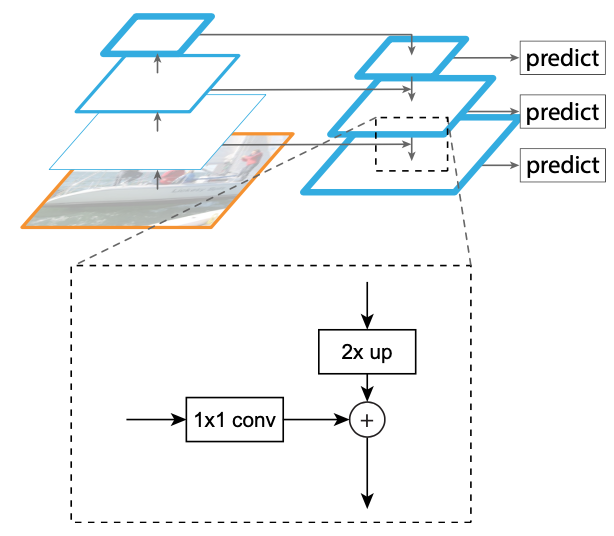
\includegraphics[width=6cm] {images/fpn_detail}
        \caption{Chi tiết kiến trúc FPN (Nguồn: \cite{lin2017feature})}
        \label{fig:fpn_detail}
    \end{figure}

    \noindent
    \textbf{\textit{Kết hợp kiến trúc mô hình FPN vào RPN}} \\

    \noindent
    \textbf{\textit{Kết hợp kiến trúc mô hình FPN vào Fast R-CNN}} \\
}